\documentclass[12pt,letterpaper,noanswers]{exam}
\usepackage[usenames,dvipsnames,svgnames,table]{xcolor}
\usepackage[margin=0.9in]{geometry}
\renewcommand{\familydefault}{\sfdefault}
\usepackage{multicol}
\usepackage{wrapfig}
\pagestyle{head}
\header{AM 22b Class 34}{}{Apr 21: Differential equations}
\runningheadrule
\headrule
\usepackage{graphicx} % more modern
\usepackage{amsmath} 
\usepackage{amssymb} 
\usepackage{hyperref}
\usepackage{tcolorbox}
\usepackage[utf8]{inputenc}
\usepackage{diagbox}
\usepackage{graphicx} 
\usepackage{enumitem}
\usepackage{tikz}
\tikzstyle{startstop} = [rectangle, rounded corners, minimum width=3cm, minimum height=1cm,text centered, draw=black]

\tikzstyle{process} = [rectangle, minimum width=3cm, minimum height=1cm, text centered, draw=black, fill=gray!20]
\tikzstyle{decision} = [ellipse, minimum width=3cm, minimum height=0.5cm, text centered, draw=black, fill=white!30]
\tikzstyle{arrow} = [thick,->,>=stealth]
\usetikzlibrary{shapes.geometric, arrows}
\pagenumbering{arabic}

\usepackage[numbered,autolinebreaks,useliterate]{mcode}

\newcommand{\mb}[1]{\underline{#1}}

\begin{document}
 \pdfpageheight 11in 
  \pdfpagewidth 8.5in




% I need to review the torus trajectories...

\begin{itemize}
% \item There is a pre-class assignment (20 minutes of videos + a few WeBWorK exercises) due at 10am this Monday.  It is available on Canvas.
\itemsep0em
\item PSet 09 is due Thurs Apr 22nd at 6pm ET.
\item Our final skill check will be on Monday (C33, 34, 35).
\item Quiz 06 will be posted on Friday.  The info is on Canvas.
\end{itemize}

\hrule
\vspace{0.2cm}

% partial derivatives, gradient
% local linearity, differential, directional deriv
% 2nd order partials + equations with partials

\noindent\textbf{Big picture}

We will learn how to analyze differential equations from three perspectives: using approximate solutions (slope fields + Euler's method + RK45), finding exact solutions (rarely, using separation of variables), using qualitative methods (identifying equilibrium solutions and whether they are `stable' or `unstable').

Today we will work with systems of equations.

\vspace{0.2cm}
\hrule
\vspace{0.2cm}


\noindent\textbf{Skill Check C34 Practice}

Sketch the phase portrait in phase space for $\dot x = x(1+x)(2+x)$.  (Construct the phase line)


\vspace{0.2cm}
\hrule
\vspace{0.2cm}

\noindent\textbf{Skill Check C34 Practice Solution}

$\dot x = 0$ for $x = 0, -1, -2$, so those are the locations with circles.

For $x > 0$, $\dot x = + + + > 0$ (the three terms of the product are each positive).

For $-1 < x < 0, \dot x = - + + < 0$.

For $-2 < x < -1, \dot x = - - + > 0$.

For $-2 < x, \dot x = - - - < 0$.

Drawing these arrows onto the line, and filling in the circle at $x = -1$, I have:


\includegraphics{img/C34skillex.pdf}

\vspace{0.2cm}
\hrule
\vspace{0.2cm}

\noindent\textbf{Teams}

\begin{multicols}{2}

1.  student names
\end{multicols}


\vspace{0.2cm}
\hrule
\vspace{0.2cm}


\noindent\textbf{Brief summary}
\begin{tcolorbox}
\begin{itemize}
\itemsep0em
    \item Differential equations can be used to model the evolution of quantities (for example, population) over time.
    \item For first order separable differential equations of the form $\frac{dx}{dt} = g(t)h(x)$, we can find a solution via separation of variables: $\displaystyle\int \frac{1}{h(x)} \frac{dx}{dt} dt = \int g(t) dt$.
    \item The solution to a differential equation may not be unique.  For example, if we encounter an empty bucket at time zero, the bucket could have become empty at any time in the past and a number of different possible solutions would describe that emptying process (each solution would differ in the time that it terminated, but each time would be before time zero).
\end{itemize}
\end{tcolorbox}

\vspace{0.2cm}
\hrule
\vspace{0.2cm}


\noindent\textbf{Problem.}  Consider the initial value problem with the logistic differential equation, $\dfrac{dx}{dt} = ax(1-x/k), x(0) = k/2$.
\begin{enumerate}
    \item Find a solution to this differential equation.
    \vspace{2.5in}
    
    \item By taking a limit, identify the long term behavior of your solution as $t\rightarrow \infty$.  In addition, identify the negative time behavior as $t\rightarrow -\infty$.
\end{enumerate}

\vfill

\vspace{0.2cm}
\hrule
\vspace{0.2cm}

\noindent\textbf{Systems of differential equations} \S 17.4
\begin{tcolorbox}
\begin{itemize}
\itemsep0em
    \item Just as we work to solve systems of equations, such at $\left\{\begin{array}{l}2x + y^2 = 7 \\ 3xy = 5\end{array}\right.$, we can work to analyze systems of first order differential equations, such as $\left\{\begin{array}{l}\dot{x} = x^2 + xy \\ \dot{y} = y-x\end{array}\right.$
    \begin{itemize}
    \itemsep0em
        \item The \textbf{order} of a differential equation is the maximum number of derivatives present in the equation.
    \item Recall that $\dot x$ and $\dot y$ are \textbf{Newton's notation} for $\frac{dx}{dt}$ and $\frac{dy}{dt}$, respectively.
    \end{itemize}
    \item The \textbf{dimension} of a system of first order ordinary differential equations is the number of equations in the system.
    \item We encountered systems of differential equations when we were solving for flow lines of a vector field.  In that case, we interpreted the vectors of the vector field as specifying the velocity of a massless particle being moved under the action of the vector field.
    \end{itemize}
    \end{tcolorbox}
    \noindent\textbf{Example: Flow lines} 
    
    Write the system of differential equations associated with the vector field $\underline F = \langle 2x + y, y - x\rangle$.
    \vfill
    
    \eject
    \vspace{0.2cm}
\hrule
\vspace{0.2cm}

    \noindent\textbf{Vocabulary: phase space, orbit}
    \begin{tcolorbox}
    \begin{itemize}
    \itemsep0em
        \item For a first order system of differential equations, the term \textbf{phase space} refers to the space of all dependent variables.  Assuming the system is autonomous, these are the variables that set the evolution rules for the system.
        \item When a solution of the system is represented in phase space, it is often referred to as an \textbf{orbit} or \textbf{trajectory} of the system.
    \end{itemize}
    \end{tcolorbox}
    \noindent\textbf{Examples: phase space}
    
    Identify the phase space for the following systems of first order differential equations.
    \begin{enumerate}
        \item $\left\{\begin{array}{l} \dot x = 2xy \\
        \dot y = 3x^2 - 1
        \end{array}\right.$
        \item $\left\{\begin{array}{l} \dot x = x + z \\
        \dot y = xy - z \\
        \dot z = xyz
        \end{array}\right.$
        \item $\dot y = 3y - 4$ \\
    \end{enumerate}
    

    \noindent\textbf{Example: representing solutions in phase space}
    \begin{tcolorbox}
    A \textbf{phase portrait} is drawn in phase space and includes representations of a qualitatively different solutions to the system.
    \end{tcolorbox}
    The slope field and the phase portrait for $\dot x = x(1-x)$ are shown below.
    \begin{itemize}
        \item Use the slope field to sketch approximate solutions of the differential equation.
        \item What information about the solutions is encoded in the phase portrait?  
        \vspace{1in}
        
        \item What do you think the circle and disk represent?
        \vspace{0.6in}
    \end{itemize}
    
    
    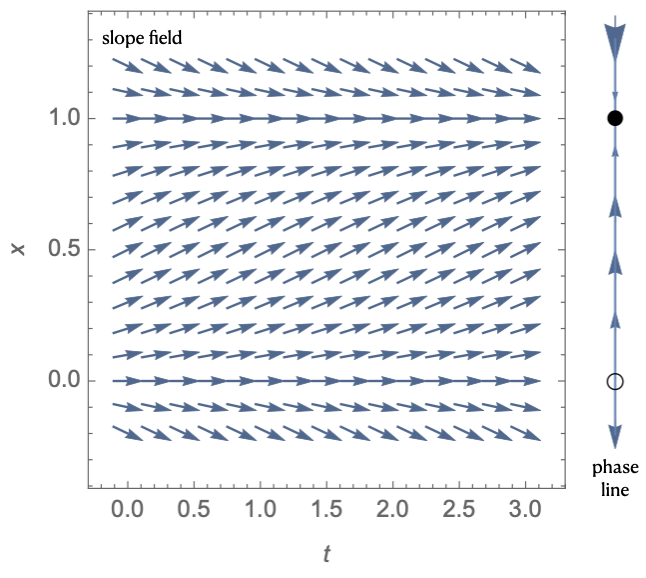
\includegraphics{img/C34slopep1b.png}
    
    A 1d phase space is called a \textbf{phase line}, and is often drawn horizontally, rather than vertically:
    
    
\includegraphics[scale=0.65]{img/C34phase1d.pdf}
    
    
    \begin{tcolorbox}
    \begin{itemize}
    \itemsep0em
    \item 
        \item The dimension of the system corresponds to the dimension of the phase space.
        \item The phase space of a single first order ODE is called the \textbf{phase line}.
        \begin{itemize}
        \itemsep0em
            \item To sketch a phase portrait on the phase line, draw a horizontal line.
            \item Identify the equilibrium solutions of $\dot x = f(x)$.  Mark them with small circles on the line.
            \item At each circle, $\dot x = 0$.  Usually, to one side of the circle, $f(x)>0$ and to the other side $f(x)<0$.  Identify the sign of $f(x)$ on either side of each circle.
            \item Draw a single arrow in the region between two circles.  If $f(x) > 0$ draw the arrow pointing right.  If $f(x)<0$, draw it pointing left.  \emph{How do you know $f(x)$ has the same sign everywhere in the region between two circles?}
            \item For circles where arrows point towards the circle from each side, fill in the circle.
        \end{itemize}
        \item The phase space of a system of two first order ODEs is called the \textbf{phase plane}.
    \end{itemize}
    \end{tcolorbox}
  %  \eject
  \noindent\textbf{Example: draw a phase portrait}
  
  Sketch the phase portrait for $\dot x = x(1+x)$.
  \vspace{1in}
    
    \noindent\textbf{Example: phase plane}
    
    Consider the system $\left\{\begin{array}{l}\dot x = x(1-x-2y) \\
    \dot y = y(1-2x-y)\end{array}\right.$
    
    The phase plane, with the vector field $\langle x(1-x-2y), y(1-2x-y)\rangle$ is shown below.
    
    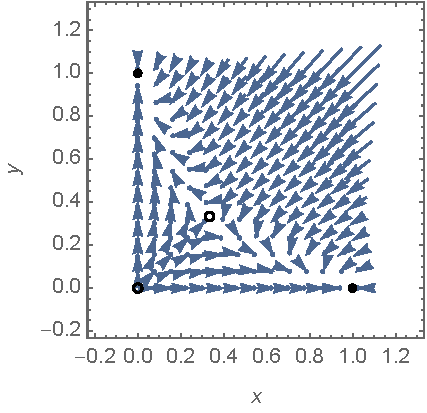
\includegraphics{img/C34phase2.pdf}
    
    \begin{itemize}
        \item From the phase plane with the vector field plotted, identify the shapes of a few flow lines.
        \vspace{1in}
        
        \item What do you think the circles and disks represent?
    \end{itemize}
    
    \vspace{0.5in}
    
    \noindent\textbf{Common examples of multi-dimensional systems}
    \begin{tcolorbox}
    \begin{itemize}
    \itemsep0em
    \item We have previously interpreted $\dot x$ and $\dot y$ as velocity information.
    \item Another common context in which systems of equations arise is the interaction of two populations.  For example, the interaction of a predator and a prey species, of two competing species, or of individuals susceptible to a disease with those infected with it.
    \item Systems of first order differential equations also arise from rewriting a higher order differential equation.  Differential equations with second derivatives often appear in physics applications, where forces produce acceleration, a second derivative of position.
    \item Systems of first order differential equations also arise in the process of approximating a system with time delay.  For example, $\dfrac{dP(t)}{dt} = aP(t-k)$ is an equation where the rate of change of the current population is proportional to the population at a time $k$ days ago (where $t$ is measured in days), rather than proportional to the current population.  
\end{itemize}
\end{tcolorbox}


\vspace{0.2cm}
\hrule
\vspace{0.2cm}



\end{document}